\documentclass[12pt]{article}
\usepackage[paperwidth=19cm, paperheight=10cm, margin=0.2cm]{geometry}
\usepackage{tikz}
\usetikzlibrary{positioning, arrows.meta, calc, decorations.pathreplacing}
\pagestyle{empty}
\setlength{\parindent}{0pt}

% ============================================================================
% COLORES Y ESTILOS
% ============================================================================
\definecolor{pastelblue}{RGB}{230, 242, 252}

\tikzset{
  box/.style={
    draw, thick, fill=pastelblue,
    minimum height=1.5cm,
    minimum width=2.0cm,
    font=\small\sffamily,
    align=center
  },
  signal/.style={-{Stealth[length=2mm]}, thick, black}, 
  lbl/.style={font=\tiny\sffamily, text=black},
  lblcenter/.style={font=\small\sffamily, align=center}
}

% Triangulo de reloj
\newcommand{\clkpin}[1]{
  \draw[thick] ([yshift=-4mm, xshift=0mm]#1.west) -- ++(2.5mm, 2.5mm) -- ++(-2.5mm, 2.5mm);
}

% MUX 2-a-1 (Select arriba)
\newcommand{\drawmux}[4]{
  \draw[thick, fill=pastelblue] (#1-0.4,#2+0.8) -- (#1+0.4,#2+0.4) -- (#1+0.4,#2-0.4) -- (#1-0.4,#2-0.8) -- cycle;
  \node[font=\tiny\sffamily] at (#1-0.15, #2+0.4) {0};
  \node[font=\tiny\sffamily] at (#1-0.15, #2-0.4) {1};
  \coordinate (#3_in0) at (#1-0.4, #2+0.4);
  \coordinate (#3_in1) at (#1-0.4, #2-0.4);
  \coordinate (#3_in2) at (#1-0.4, #2); 
  \coordinate (#3_out) at (#1+0.4, #2);
  \coordinate (#3_sel) at (#1, #2+0.6);
}

% MUX 2-a-1 (Select abajo)
\newcommand{\drawmuxdown}[3]{
  \draw[thick, fill=pastelblue] (#1-0.4,#2+0.8) -- (#1+0.4,#2+0.4) -- (#1+0.4,#2-0.4) -- (#1-0.4,#2-0.8) -- cycle;
  \node[font=\tiny\sffamily] at (#1-0.15, #2+0.4) {0};
  \node[font=\tiny\sffamily] at (#1-0.15, #2-0.4) {1};
  \coordinate (#3_in0) at (#1-0.4, #2+0.4);
  \coordinate (#3_in1) at (#1-0.4, #2-0.4);
  \coordinate (#3_out) at (#1+0.4, #2);
  \coordinate (#3_sel) at (#1, #2-0.6);
}

% Adder
\newcommand{\drawadder}[3]{
  \draw[thick, fill=pastelblue] 
    (#1-0.6, #2+1.0) -- 
    (#1-0.6, #2+0.2) -- 
    (#1-0.3, #2) -- 
    (#1-0.6, #2-0.2) -- 
    (#1-0.6, #2-1.0) -- 
    (#1+0.6, #2-0.5) -- 
    (#1+0.6, #2+0.5) -- cycle;
  \node[font=\small\sffamily] (#3) at (#1+0.1, #2) {$+$};
  \coordinate (#3_in1) at (#1-0.6, #2+0.5);
  \coordinate (#3_in2) at (#1-0.6, #2-0.5);
  \coordinate (#3_out) at (#1+0.6, #2);
}

\begin{document}
\noindent
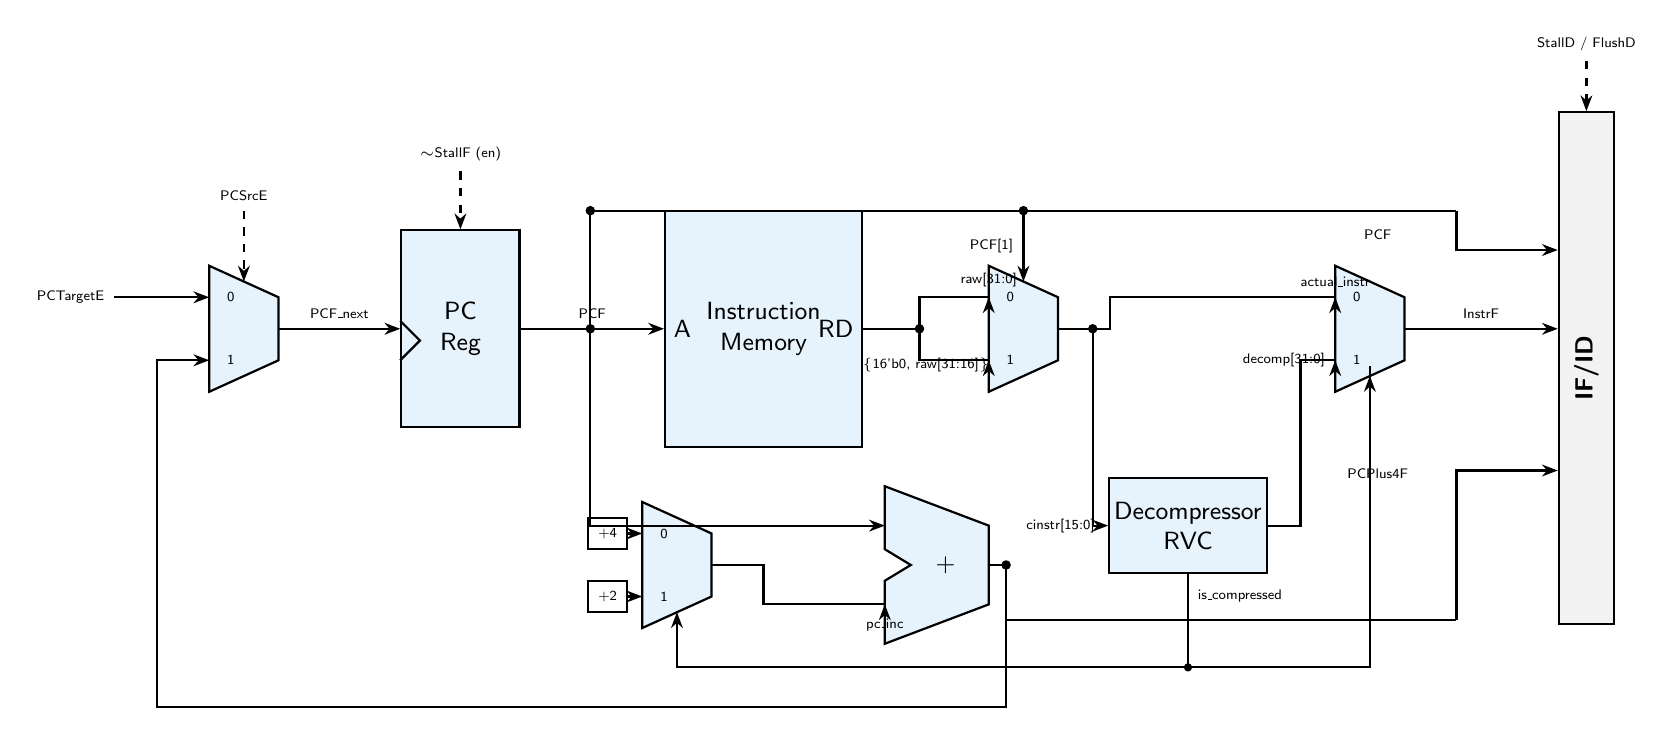
\begin{tikzpicture}[
  x=1.1cm, y=1.0cm,
  signal/.style={-{Stealth[length=2mm]}, thick, black},
  lbl/.style={font=\tiny\sffamily, text=black},
  lblcenter/.style={font=\small\sffamily, align=center},
]

  % ============================================================================
  % COMPONENTES DE LA LINEA PRINCIPAL (y = 1.0)
  % ============================================================================

  % 1. MUX del PC (pcmux)
  \drawmux{-4.5}{1.0}{pcmux}{MUX PC}
  
  \draw[signal] (-6.0, 1.4) -- (pcmux_in0);
  \node[left, lbl] at (-6.0, 1.4) {PCTargetE};

  % 2. Registro PC
  \node[box, minimum height=2.5cm, minimum width=1.5cm] (pcreg) at (-2.0, 1.0) {};
  \node[lblcenter] at (-2.0, 1.0) {PC\\Reg};
  \clkpin{pcreg}

  % 3. Memoria de Instrucciones (IMEM)
  \node[box, minimum height=3.0cm, minimum width=2.5cm] (imem) at (1.5, 1.0) {};
  \node[lblcenter] at (1.5, 1.0) {Instruction\\Memory};
  \node[font=\small\sffamily, right] at (imem.west |- {0,1}) {A};
  \node[font=\small\sffamily, left] at (imem.east |- {0,1}) {RD};

  % 4. MUX de Alineacion (alignmux)
  \drawmux{4.5}{1.0}{alignmux}{MUX Align}

  % 5. MUX Final de Instruccion (instrmux) - Select abajo
  \drawmuxdown{8.5}{1.0}{instrmux}{MUX Inst}

  % 6. Registro de Pipeline IF/ID (vertical gray bar)
  \node[draw, fill=gray!10, thick, minimum width=0.7cm, minimum height=6.5cm, font=\small\sffamily\bfseries] (ifid) at (11.0, 0.5) {\rotatebox{90}{IF/ID}};

  % ============================================================================
  % CONEXIONES DE LA LINEA PRINCIPAL
  % ============================================================================
  
  % pcmux a PC Reg
  \draw[signal] (pcmux_out) -- (pcreg.west) node[midway, above, lbl] {PCF\_next};
  
  % PC Reg a IMEM
  \draw[signal] (pcreg.east) -- (imem.west |- {0,1}) node[midway, above, lbl] {PCF};

  % IMEM a alignmux (in0)
  \draw[thick] (imem.east |- {0,1}) -- (3.3, 1.0) |- (alignmux_in0);
  \draw[signal] (alignmux_in0) -- (alignmux_in0) node[lbl, pos=0.2, above] {raw[31:0]};

  % Derivacion para la mitad superior desalineada (in1)
  \draw[fill=black] (3.3, 1.0) circle (1.5pt);
  \draw[thick] (3.3, 1.0) |- (3.3, 0.6) -- (4.1, 0.6);
  \draw[signal] (4.1, 0.6) -- (alignmux_in1);
  \node[below, lbl, xshift=-0.8cm, yshift=0.15cm] at (alignmux_in1) {\{16'b0, raw[31:16]\}};

  % alignmux a instrmux (in0)
  \draw[thick] (alignmux_out) -- (5.5, 1.0) |- (8.1, 1.4);
  \draw[signal] (8.1, 1.4) -- (8.1, 1.4) node[lbl, pos=0.2, above] {actual\_instr};

  % instrmux a IF/ID
  \draw[signal] (instrmux_out) -- (ifid.west |- {0, 1.0}) node[midway, above, lbl] {InstrF};

  % ============================================================================
  % CAMINO DEL DESCOMPRESOR RVC (y = -1.5)
  % ============================================================================

  % Descompresor RVC
  \node[box, minimum width=2.0cm, minimum height=1.2cm] (decomp) at (6.4, -1.5) {};
  \node[lblcenter] at (6.4, -1.5) {Decompressor\\RVC};

  % Tap de actual_instr hacia decompressor input
  \draw[fill=black] (5.3, 1.0) circle (1.5pt);
  \draw[thick] (5.3, 1.0) -- (5.3, -1.5);
  \draw[signal] (5.3, -1.5) -- (decomp.west) node[lbl, pos=0.8, left] {cinstr[15:0]};

  % Salida del descompresor a instrmux_in1
  \draw[thick] (decomp.east) -- (7.7, -1.5) |- (8.1, 0.6);
  \draw[signal] (8.1, 0.6) -- (instrmux_in1) node[lbl, pos=0.2, left] {decomp[31:0]};

  % Senal is_compressed
  \draw[thick] (decomp.south) -- (6.4, -3.3);
  \node[right, lbl] at (6.4, -2.4) {is\_compressed};
  \fill (6.4, -3.3) circle (1.5pt);

  % Conectar is_compressed a instrmux_sel (abajo)
  \draw[thick] (6.4, -3.3) -- (8.5, -3.3) -- (8.5, 0.4);
  \draw[signal] (8.5, 0.4) -- (instrmux_sel);

  % ============================================================================
  % CAMINO DE INCREMENTO DINAMICO DEL PC (y = -2.0)
  % ============================================================================

  % Mux de Incremento (incmux) - Select abajo
  \drawmuxdown{0.5}{-2.0}{incmux}
  
  \node[draw, thick, fill=white, minimum width=0.5cm, minimum height=0.4cm, font=\tiny\sffamily] (c4) at (-0.3, -1.6) {+4};
  \node[draw, thick, fill=white, minimum width=0.5cm, minimum height=0.4cm, font=\tiny\sffamily] (c2) at (-0.3, -2.4) {+2};
  \draw[signal] (c4.east) -- (incmux_in0);
  \draw[signal] (c2.east) -- (incmux_in1);

  % Conectar is_compressed a incmux_sel (abajo)
  \draw[signal] (6.4, -3.3) -- (0.5, -3.3) -- (incmux_sel);

  % Sumador del PC (pcadd)
  \drawadder{3.5}{-2.0}{pcadd}

  % Conectar pc_increment a pcadd_in2
  \draw[thick] (incmux_out) -- (1.5, -2.0) |- (2.9, -2.5);
  \draw[signal] (2.9, -2.5) -- (pcadd_in2) node[midway, below, lbl, yshift=-0.05cm] {pc\_inc};

  % Conectar PCF a pcadd_in1
  \draw[fill=black] (-0.5, 1.0) circle (1.5pt);
  \draw[signal] (-0.5, 1.0) |- (pcadd_in1);

  % ============================================================================
  % BUSES E HILOS GLOBALES
  % ============================================================================

  % Retorno PCPlus4F
  \draw[fill=black] (4.3, -2.0) circle (1.5pt);
  \draw[thick] (pcadd_out) -- (4.3, -2.0);
  
  % Lazo de feedback inferior a pcmux_in1
  \draw[signal] (4.3, -2.0) |- (4.3, -3.8) -- (-5.5, -3.8) |- (-5.5, 0.6) -- (pcmux_in1);

  % PCPlus4F a IF/ID (entrada de retorno inferior)
  \draw[thick] (4.3, -2.0) |- (4.3, -2.7) -- (9.5, -2.7);
  \draw[signal] (9.5, -2.7) |- (ifid.west |- {0, -0.8}) node[midway, below, lbl, xshift=-1cm, yshift=0.15cm] {PCPlus4F};

  % PCF a IF/ID (entrada de PCF superior)
  \draw[fill=black] (-0.5, 2.5) circle (1.5pt);
  \draw[thick] (-0.5, 1.0) -- (-0.5, 2.5) -- (9.5, 2.5);
  \draw[signal] (9.5, 2.5) |- (ifid.west |- {0, 2.0}) node[midway, above, lbl, xshift=-1cm] {PCF};

  % Tap de PCF[1] a alignmux_sel
  \draw[fill=black] (4.5, 2.5) circle (1.5pt);
  \draw[signal] (4.5, 2.5) -- (alignmux_sel) node[midway, left, lbl] {PCF[1]};

  % ============================================================================
  % LINEAS DE CONTROL Y RELOJ (Dashed)
  % ============================================================================

  % PCSrcE
  \draw[signal, dashed] (-4.5, 2.5) node[above, lbl] {PCSrcE} -- (pcmux_sel);

  % StallF
  \draw[signal, dashed] (-2.0, 3.0) node[above, lbl] {$\sim$StallF (en)} -- (pcreg.north);

  % Control de IF/ID (StallD / FlushD)
  \draw[signal, dashed] (11.0, 4.4) node[above, lbl] {StallD / FlushD} -- (ifid.north);

\end{tikzpicture}
\end{document}
